The crossover Core is the next part in the genetics accelerator after the selection cores.
Two inputs are forwarded from the two selections cores as "parents", and two outputs are the "children" of the inputs, containing bits from both parents.
All the bits from both the parents are forwarded in the children, but in some parts the bit-patterns are switched on the children, based a selected crossover function and on a random input from the PRNG.
Henceforth this is called crossover.

There are three distinct crossover functions that are implented: Split, double-split and XOR.


\paragraph{\textit{Split Fucntion}}
\begin{figure}[H]
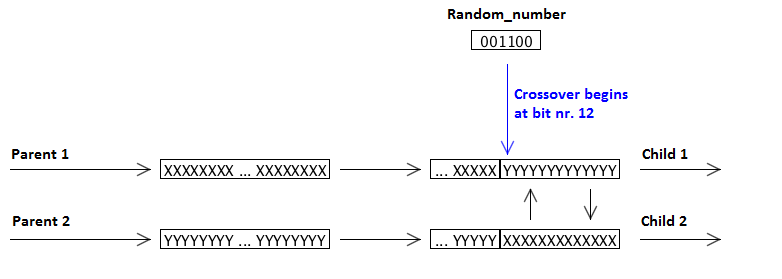
\includegraphics[width=\textwidth]{fpga/fig/crossover_split.png}
\caption{Crossover split function}
\label{fig_crossover_split}
\end{figure}

The first function, crossover split, performs crossover from a selected bit number in the children and until the edge (which is bit number 0).
This can be seen in figure \ref{fig_crossover_split}.
The values in the parents are represented with X's and Y's, and a single X or Y can have the value 0 or 1, independent of each other.
The bit number for starting crossover is based on the value of a 6-bit input random\_number, which is provided by the PRNG. 
This value ranges from 0 to 63. 
Figure \ref{fig_crossover_split} uses the value 001100 as example, and the selected bit number is 12. 
The function will perform crossover on bits 12-0 in the children.

\begin{figure}[H]
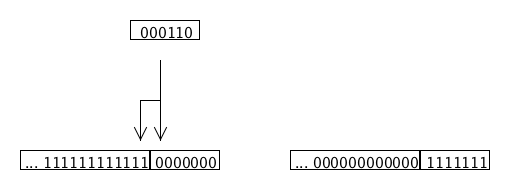
\includegraphics[width=\textwidth]{fpga/fig/crossover_split_mask.png}
\caption{Masking for split function}
\label{fig_crossover_split_mask}
\end{figure}

The split function was originally implemented by using behavioural descpription, but this caused the synthesizer to create many latches.
The same problem occured also for the double-split function.
In order to avoid this, the function now uses a ShifterVariable, that uses a 32-bit number of 1's as main input, and the random\_number for shifting input.
This yields an output that consists of 1's until the selected bit number, and 0's on the rest.
Figure \ref{fig_crossover_split_mask} shows an example where bit number 6 is selected for where to begin crossover. 
Bits 6-0 in the output consist of 0's, and the rest 1's.
This output is called \emph{mask1}. Notice that \emph{mask1} has had an extra shift to the left, in order to perform the crossover from the correct selected bit. 
The ShifterVariable performs shifting with an input of 1's, and in this example bit number 6 would be the last bit with value 1, but it needs to be the first bit with value 0. Therefore, an extra shift is required.
\todo{ Hmm....mulig det trengs å beskrives om ShifterVariables snart, så at denne beskrivelsen kan forbedres. Btw: THE CAKE IS A LIE!!}
\emph{Mask2} is set as a negation of \emph{mask1}, so the bits in \emph{mask2} would be 1's where they would be 0's in \emph{mask1}, and vice versa.
Only bits 6-0 would be 1's in \emph{mask2} in the figure.
The output on the children are set by combininging the parents and the masks:
\linebreak
\linebreak child1 $\leftarrow$ (parent1 and mask1) or (parent2 and mask2);
\linebreak child2 $\leftarrow$ (parent1 and mask2) or (parent2 and mask1);
\linebreak \todo{ ShifterVariable needs to be described.}

\paragraph{\textit{Double-split Fucntion}}
\begin{figure}[H]
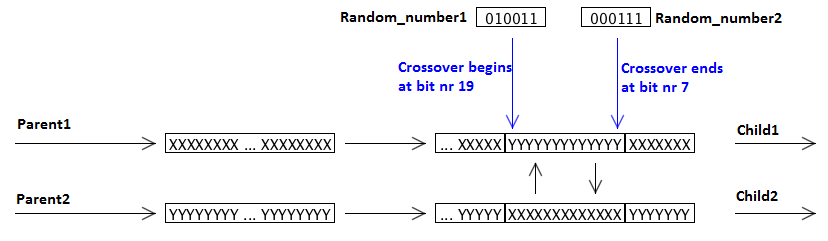
\includegraphics[width=\textwidth]{fpga/fig/crossover_doublesplit.png}
\caption{Crossover double-split function}
\label{fig_crossover_doublesplit}
\end{figure}

The second function, crossover double-split, is similar to the split function, but in addition to having a starting bit for crossover, it also has an ending bit where the crossover ends, instead of reaching the edge at bit number 0.
PRNG provides with 2 6-bit inputs, \emph{random\_number1} and \emph{random\_number2}, which values select the starting bit and the ending bit for the crossover.
These values range from 0 to 63, and if both are the same, then crossover will only be performed on one bit.

\begin{figure}[H]
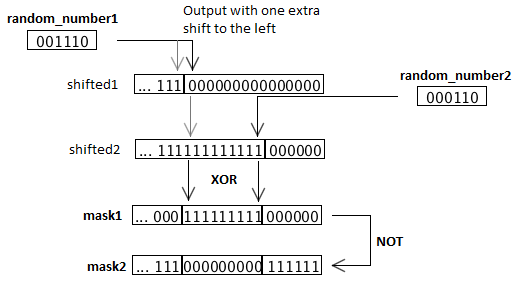
\includegraphics[width=\textwidth]{fpga/fig/crossover_doublesplit_mask2.png}
\caption{Masking for double-split function}
\label{fig_crossover_doublesplit_mask}
\end{figure}

The double-split function uses two ShifterVariables, which take an input each from the random\_numbers.
The ShifterVariables are used in the same way as in the split function, but the outputs will differ from each other as to where the transition from 1's to 0's are set.
One will have more 1's than the other (at least one if both the random numbers are the same).
The masks are set by using XOR-function of these outputs, so that \emph{mask1} will have 0's in both the MS and the LS portions of bits, but with a area of 1's between, and \emph{mask2} is it's negation.
Figure \ref{fig_crossover_doublesplit_mask} provides such an example, where bits number 14 and 6 are selected.
The bits 14-6 in \emph{mask1} would be 1's and the rest 0's by using XOR-function with the outputs from the ShifterVariables, and vice versa in \emph{mask2} by setting it as the negation of \emph{mask1}.
The final outputs are set the same way as in the split function.

\todo{ ShifterVariable needs to be described.}

\paragraph{\textit{XOR Function}}
\begin{figure}[H]
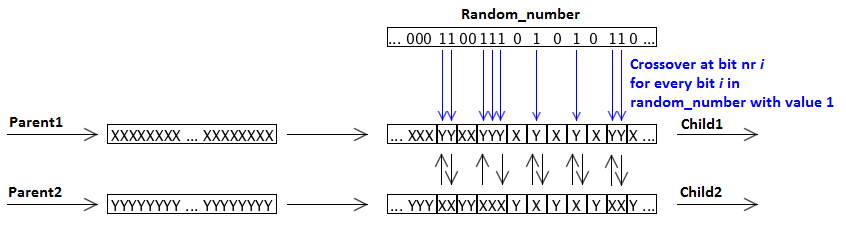
\includegraphics[width=\textwidth]{fpga/fig/crossover_xor.png}
\caption{Crossover XOR function}
\label{fig_crossover_xor}
\end{figure}

The third function, crossover XOR, performs crossover bit by bit, based on the 64-bit input random\_number.
For each bit number \emph{i} in random\_number that has the value 1, the function will perform crossover on the children at the same bit number \emph{i}.
This function is called XOR because of use of XOR-gates in earlier version of the function, and the principle is still the same: For each bit number \emph{i} in the child, the value will the bit number \emph{i} from one and only one parent.
And which parent it is depends on the value of bit number \emph{i} in random\_number.

\paragraph{\textit{Crossover Core Toplevel}}
\todo{ Bilde hadde vært fint, men teksten er klar nok til at det trolig går an å droppe hvis det ikke blir tid. Foreslår å nedprioritere}
The crossover core is implemented on the genetics accelerator as a toplevel containing 3 subcores, one for each function, as well as a fourth path with no crossover.
In addition to the two parent inputs and 64-bit input random\_number, the toplevel has a control\_number input used for determining which crossover function is to be used: Split, doublesplit, xor, "party mode" or no crossover at all.
Party mode is choosing crossover function at random, based on the 2 LS bits in the random\_number.
In this way, whenever inputs are sent through the crossover\_toplevel, different functions may be used at different times.
These are the control values:
\begin{itemize}
\item 000 - Split
\item 001 - Double-split
\item 010 - XOR
\item 011 - No crossover
\item 1XX - Party mode, in which case these are the random control values:
    \begin{itemize}
    \item 00 - Split
    \item 01 - Doublesplit
    \item 10 - XOR
    \item 11 - No crossover
    \end{itemize}
\end{itemize}
